\chapter{寻找巨洞及巨洞的统计性质}
\label{cha:DIVE}

\section{引言}

德劳内三角剖分~\cite{Delaunay1934}(Delaunay Triangulation,DT)被广泛用于天文学研究中~\cite{Bernardeau1996,Marinoni2002,Pal2006,Cardiel2001,Weygaert2011,Berge2012,Cedres2012}。文献 ~\inlinecite{Schaap2000} 开发了可以利用离散的样本重构连续密度场的Delaunay tessellation field estimator(DTFE),在此基础之上从理论和观测上研究宇宙大尺度结构~\cite{Aragon-Calvo2007,Romano-Diaz2007,Weygaert2009,Platen2011,Sousbie2011,Jennings2012}。文献 ~\inlinecite{Platen2007} 在DTFE的基础上开发了The Watershed Void Finder(WVF),文献 ~\inlinecite{Neyrinck2008}基于Voronoi Diagram开发了ZOBOV,文献 ~\inlinecite{Sutter2015VIDE}对ZOBOV的功能做了一些扩展和强化开发出VIDE。文献 ~\inlinecite{Gaite2005}和文献 ~\inlinecite{Way2015}直接将DT所得到的空心四面体定义为巨洞。

我们把巨洞定义为通过星系分布找到的空心四面体所确定的空心球,并通过DIVE ~\cite{Zhao2016DIVE}对三维空间中星系的分布做DT得到空心四面体,再计算其对应空心球的中心位置和半径,因而这些空心球被称为DT巨洞。DIVE可以非常高效的从离散分布的天体中寻找所有的空心球,因此我们能够将DIVE用于100组实空间和红移空间完整模拟暗物质晕表,并分析巨洞的统计性质。在没有特别声明使用的是红移空间完整模拟暗物质晕表的情况下,都默认是实空间完整模拟暗物质晕表。

根据巨洞的统计性质可以将DT巨洞分为两类。一类相当于星系群,对应\textit{voids-in-clouds}~\cite{SW04}类巨洞,通常半径比较小,中心在高密度区域。另一类是真正宇宙学意义上的巨洞,半径比较大,占据了宇宙中低密度区域,其中的物质朝远离巨洞中心的方向运动,对应\textit{voids-in-voids}~\cite{SW04}类巨洞。

DT巨洞可以互相重叠,而文献 ~\inlinecite{Patiri2006372,VBT12,CC13}中所定义的巨洞不能互相重叠,从DT巨洞中同样可以选出不互相重叠的巨洞子样本(disjoint voids,disjoint巨洞)。本章也比较了DT巨洞和disjoint巨洞之间的差异。

通过计算DT巨洞的潮汐张量(tidal field tensor)能从动力学角度将所有DT巨洞分为宇宙大尺度结构中的不同成分。研究结果表明半径大的巨洞内部的物质都在朝远离巨洞中心的方向运动,这些巨洞都在不断变大。这一结果也表明了半径大的巨洞在低密度区域。

最后计算了不同大小的DT巨洞的功率谱,并发现两类巨洞的偏袒不同,说明两类巨洞分布在不同的大尺度结构中。

\begin{figure}
\centering
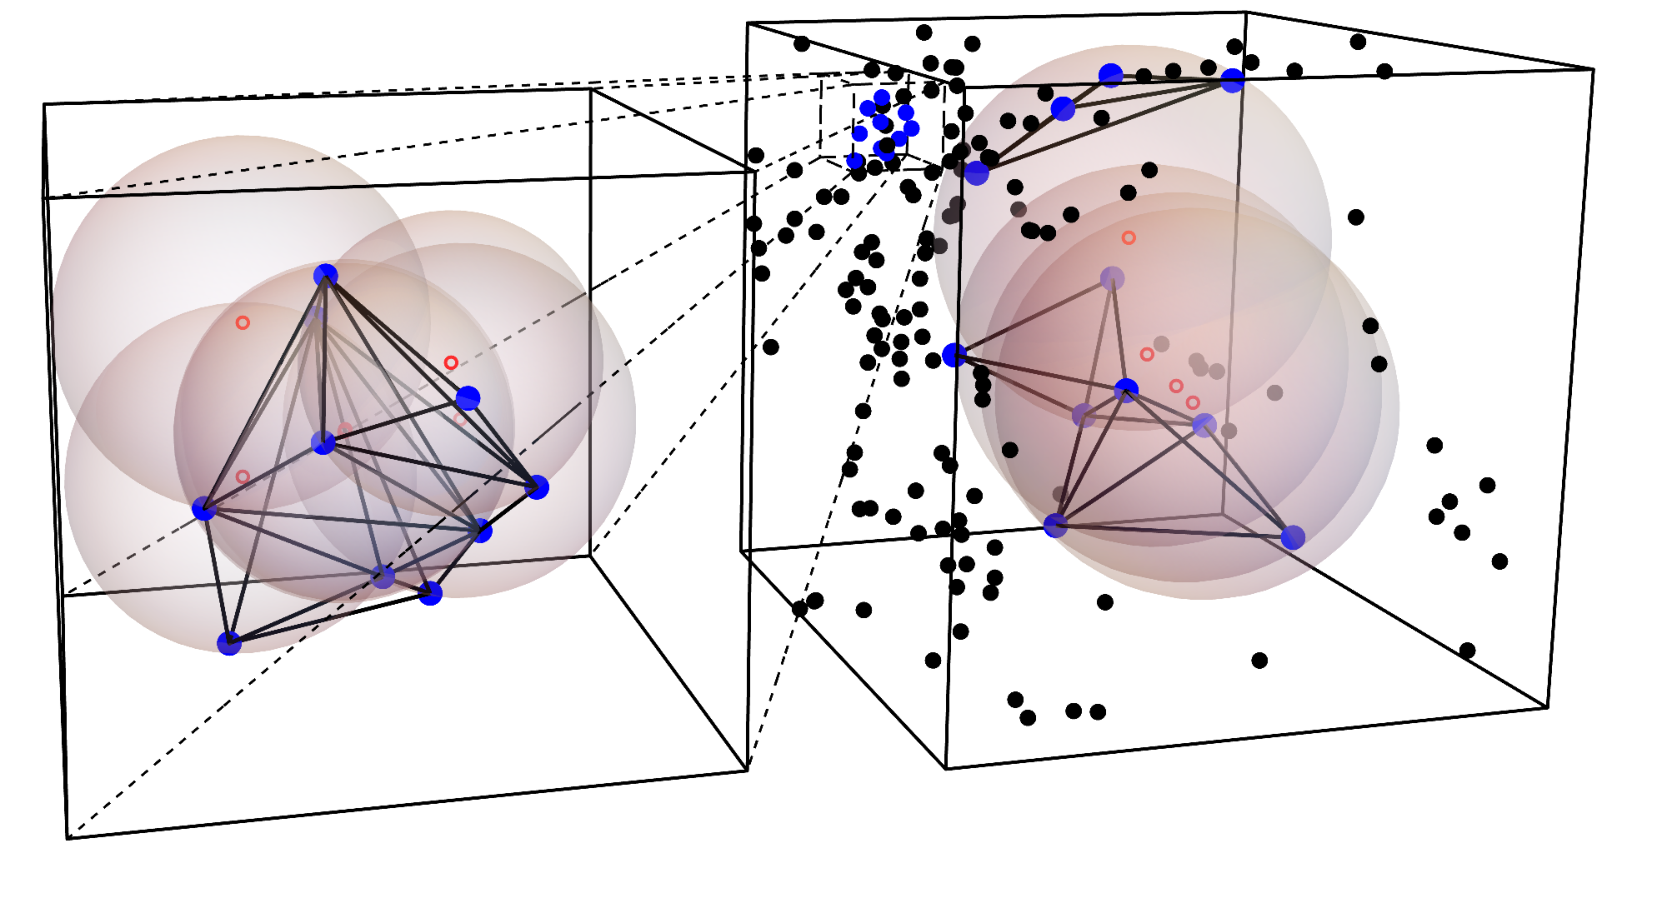
\includegraphics[width=.9\textwidth]{DTVoid_box}
\caption{完整模拟暗物质晕表中部分区域内DT巨洞和暗物质晕的相对空间分布。红色空心圆点是巨洞的中心,阴影区域表示了巨洞半径范围内的体积,DIVE找到的每个空心四面体的顶点是暗物质晕所在的位置由蓝色实心圆点表示,黑色直线表示四面体的边。左图:$12^3\,h^{-3}\mathrm{Mpc}^3$体积内半径$R \leq 4\,h^{-1}$Mpc的DT巨洞。右图:$80^3\,h^{-3}\mathrm{Mpc}^3$体积内半径$R \in [26, 27]\,h^{-1}$Mpc的DT巨洞(文献 ~\inlinecite{Zhao2016DIVE}中的Figure 1)}
\label{fig:visual_all}
\end{figure}

\section{DIVE:Delaunay trIangulation Void findEr}
\label{sec:DIVE}

DIVE可以对在三维空间中离散分布的物体,如暗物质晕或星系,做徳劳内三角剖分得到空心四面体,四面体的顶点是暗物质晕或星系所在的位置。通过四面体四个顶点可以唯一的确定一个空心球,并计算得到空心球的中心和半径。DIVE利用开源的Computational Geometry Algorithms Library\footnote{\url{http://www.cgal.org}} ~\cite{Bronnimann2015, Jamin2015}(\textsc{cgal})实现对空间的徳劳内三角剖分并计算空心球的圆心和半径。图~\ref{fig:visual_all} 展示了完整模拟暗物质晕表中一小块区域内,DT巨洞与暗物质晕在空间中的相对分布。半径较大的DT巨洞分布在空的区域,属于\textit{voids-in-voids},而半径较小的DT巨洞在许多暗物质晕中间,属于对应\textit{voids-in-clouds}。相比\textit{voids-in-voids},\textit{voids-in-clouds}对散射噪声(shot noise)更敏感~\cite{Cai2014}。

\textsc{cgal}自身没有任何参数,所以不依赖具体具体宇宙学模型。观测数据所在的空间十分不规则,但\textsc{cgal}对任意形状空间内离散分布的物体都可以进行DT。同时\textsc{cgal}的效率非常高,所以我们得以将其用于大量的完整模拟暗物质晕表进行统计分析。

\begin{figure}
\centering
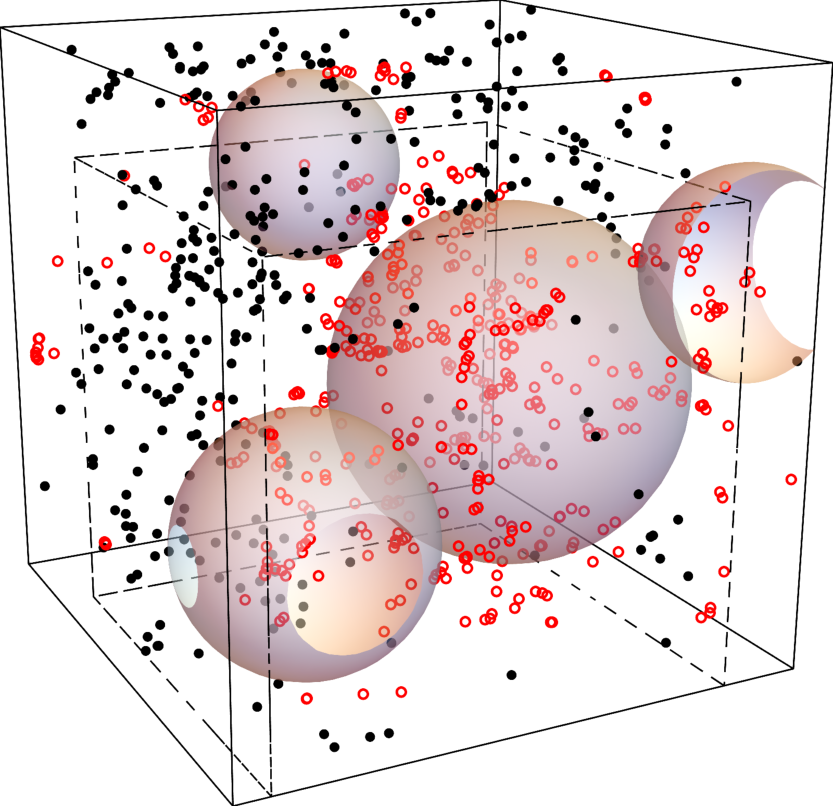
\includegraphics[width=.9\textwidth]{DTVoid_nonoverlap}
\caption{完整模拟暗物质晕表的$100^3\,h^{-3}\mathrm{Mpc}^3$部分体积内,半径$R \geq 17\,h^{-1}$Mpc的disjoint巨洞的空间分布。红色空心圆是空间内DT巨洞的球心,虚线表示的方形图~\ref{fig:visual_all} 内的区域,阴影区域是所有disjoint巨洞所占据的体积。(文献 ~\inlinecite{Zhao2016DIVE}中的Figure 2)}
\label{fig:visual_dj}
\end{figure}

使用类似HB void finder~\cite{Patiri2006372}的方法可以从DT巨洞中选出disjoint巨洞。这类巨洞与之前大部分定义的巨洞的方式类似,都不允许巨洞之间互相重叠~\cite{Patiri2006HB,Micheletti02014},因而这类巨洞的数密度会显著小于同样大小的DT巨洞。图~\ref{fig:visual_dj} 展示了一个完整模拟暗物质晕表的一部分空间内的disjoint巨洞的分布,从图中以及与图~\ref{fig:visual_all} 的对比可以看出disjoint巨洞的数密度远小于DT巨洞。

如果认为DT巨洞之间有从属关系,disjoint巨洞可以被认为是独立的巨洞(distinct巨洞、parent巨洞),与distinct巨洞重叠的巨洞是这个distinct巨洞的从属巨洞或子巨洞(subvoids)。文献 ~\inlinecite{SW04}就巨洞的从属关系也进行过研究。图~\ref{fig:subvoid} 展示了不同半径的独立巨洞的子巨洞的数量和大小的分布。可以看出更大的独立巨洞倾向于拥有更多并且更大的子巨洞。在一个较大独立巨洞所在的低密度区域内,可以存在非常多与这个独立巨洞半径大小相当的DT巨洞。同一个低密度区域内大量的DT巨洞使得更大的低密度区域拥有更大的权重。

\begin{figure}
\centering
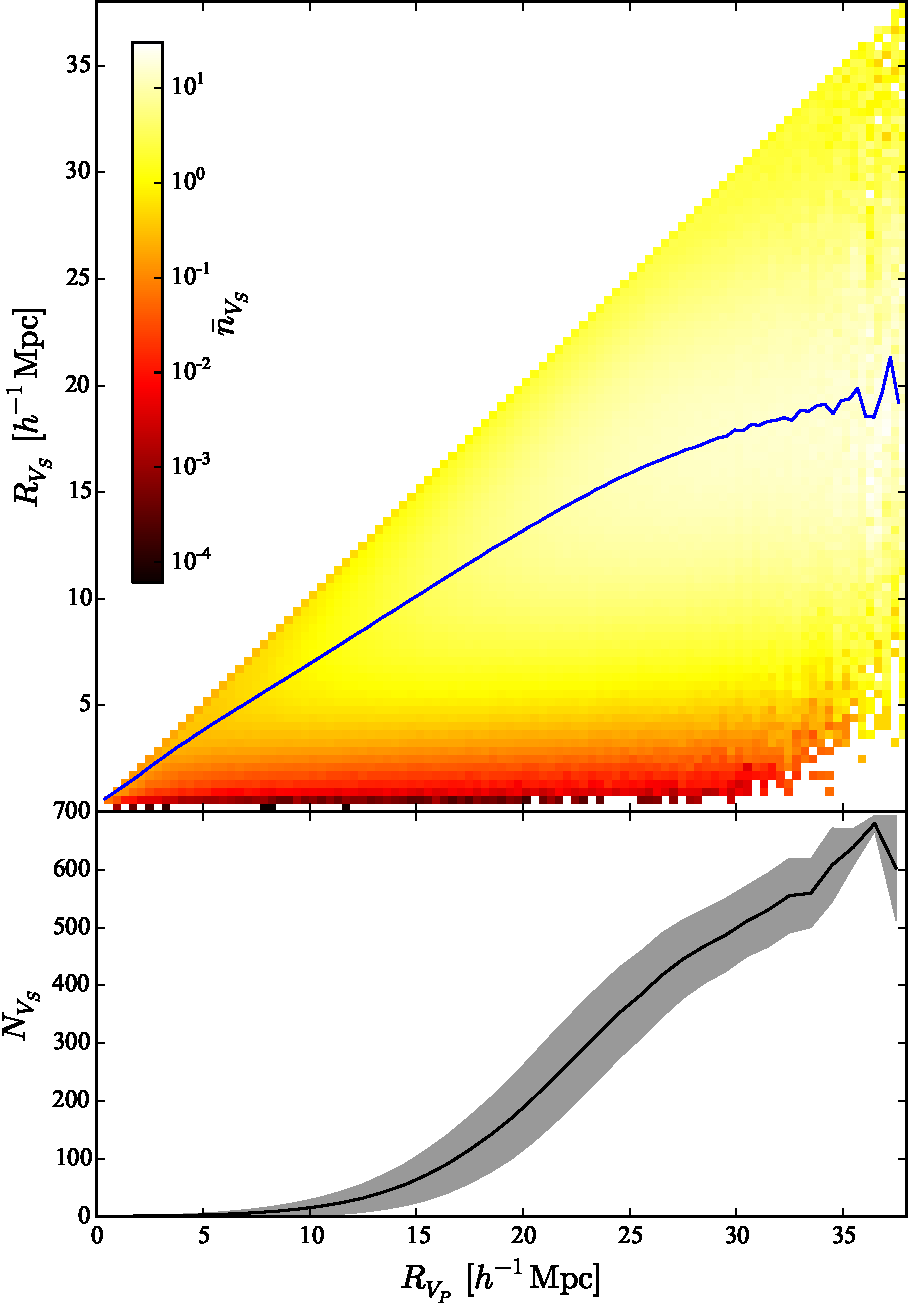
\includegraphics[width=.9\textwidth]{subvoid}
\caption{不半径独立巨洞的子巨洞的数目和半径大小的分布。上图:半径为$R_{V_P}$的独立巨洞的子巨洞的半径$R_{V_S}$分布(颜色深浅表示数目多少),蓝色实线表示子巨洞的平均半径。下图:半径为$R_{V_P}$的独立巨洞的子巨洞的平均数量$N_{V_S}$(黑色实线),和1$\sigma$误差范围(灰色区域)。结果来自一个\textsc{PATCHY}完整模拟暗物质晕表。(文献 ~\inlinecite{Zhao2016DIVE}中的Figure 7)}
\label{fig:subvoid}
\end{figure}

\section{巨洞的数密度}
\label{sec:voidnumberdensity}

巨洞的数密度是巨洞非常重要的一个性质,它决定了巨洞其他统计性质的统计显著性。同时巨洞的数密度分布也可以直接用于限制宇宙学参数~\cite{Patiri2006HB,JLH13}、研究暗能量模型~\cite{Pisani2015PRD,Sutter2015}或研究不同的引力理论~\cite{Cai2015}。

DT巨洞的一大优势就是拥有较大的数密度,结果在统计上更可靠。但DT巨洞是从空间中离散分布的暗物质晕或星系中通过DIVE获得的,其数密度分布肯定在一定程度上依赖于空间中暗物质晕或星系的数密度。实空间和红移空间完整模拟暗物质晕表的数密度都是$3.5\times10^{-4}\,h^{3}\,\mathrm{Mpc}^{-3}$,这是BOSS CMASS样本的LRG平均数密度,有些红移处的LRG数密度低于这个值。因此,我们将完整模拟暗物质晕表内的暗物质晕随机移除一部分,得到三组数密度更低([2, 2.5, 3] $\times 10^{-4}\,h^3\,\mathrm{Mpc}^{-3}$)的完整模拟暗物质晕表。

研究结果表明,随着完整模拟暗物质晕表内暗物质晕数密度的减少DT巨洞的总数也随之显著减少,但是半径$R > 16$ $h^{-1}$ Mpc的DT巨洞总数几乎保持不变,半径$R > 20$ $h^{-1}$ Mpc的巨洞数量增多,同时半径$R < 10$ $h^{-1}$ Mpc的巨洞数量减少(图~\ref{fig:ndens_nmean} 右半部分)。以此可以将DT巨洞分为两类,一类跟暗物质晕正相关,另一类与暗物质晕反相关,两类巨洞的分界线在$R \sim 16$ $h^{-1}$ Mpc。对于disjoint巨洞来说,这一分界位于$R \sim 17.5$ $h^{-1}$ Mpc,与文献 ~\inlinecite{Hamaus2014}的结果($R \sim 17.6$ $h^{-1}$ Mpc)非常接近。

\begin{figure}
\begin{tabular}{cc}
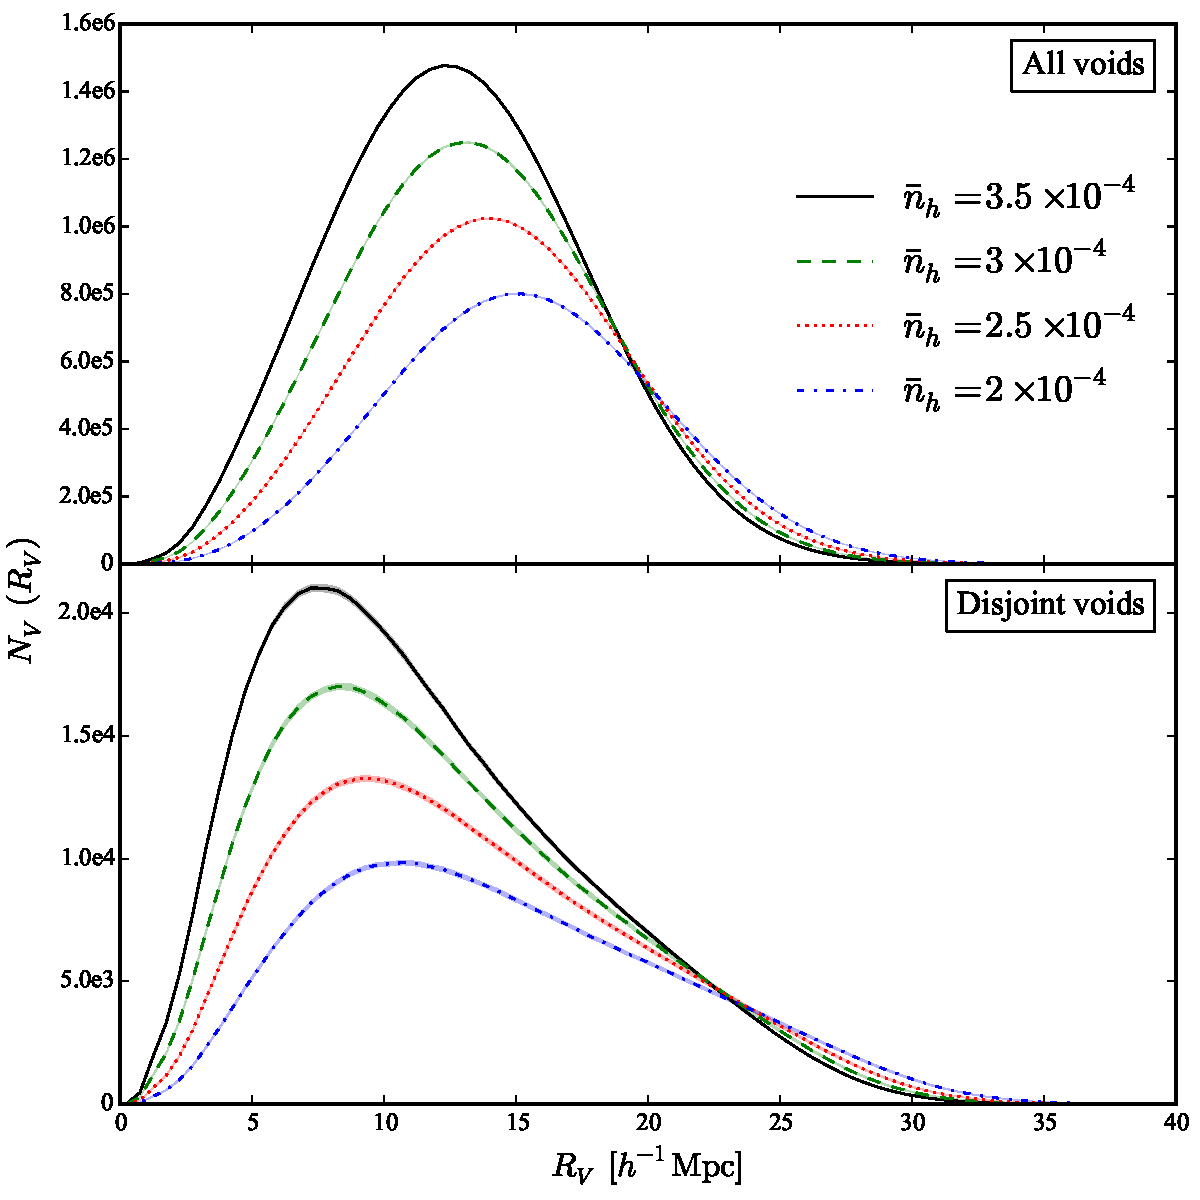
\includegraphics[width=.47\textwidth]{numdens_nmean}
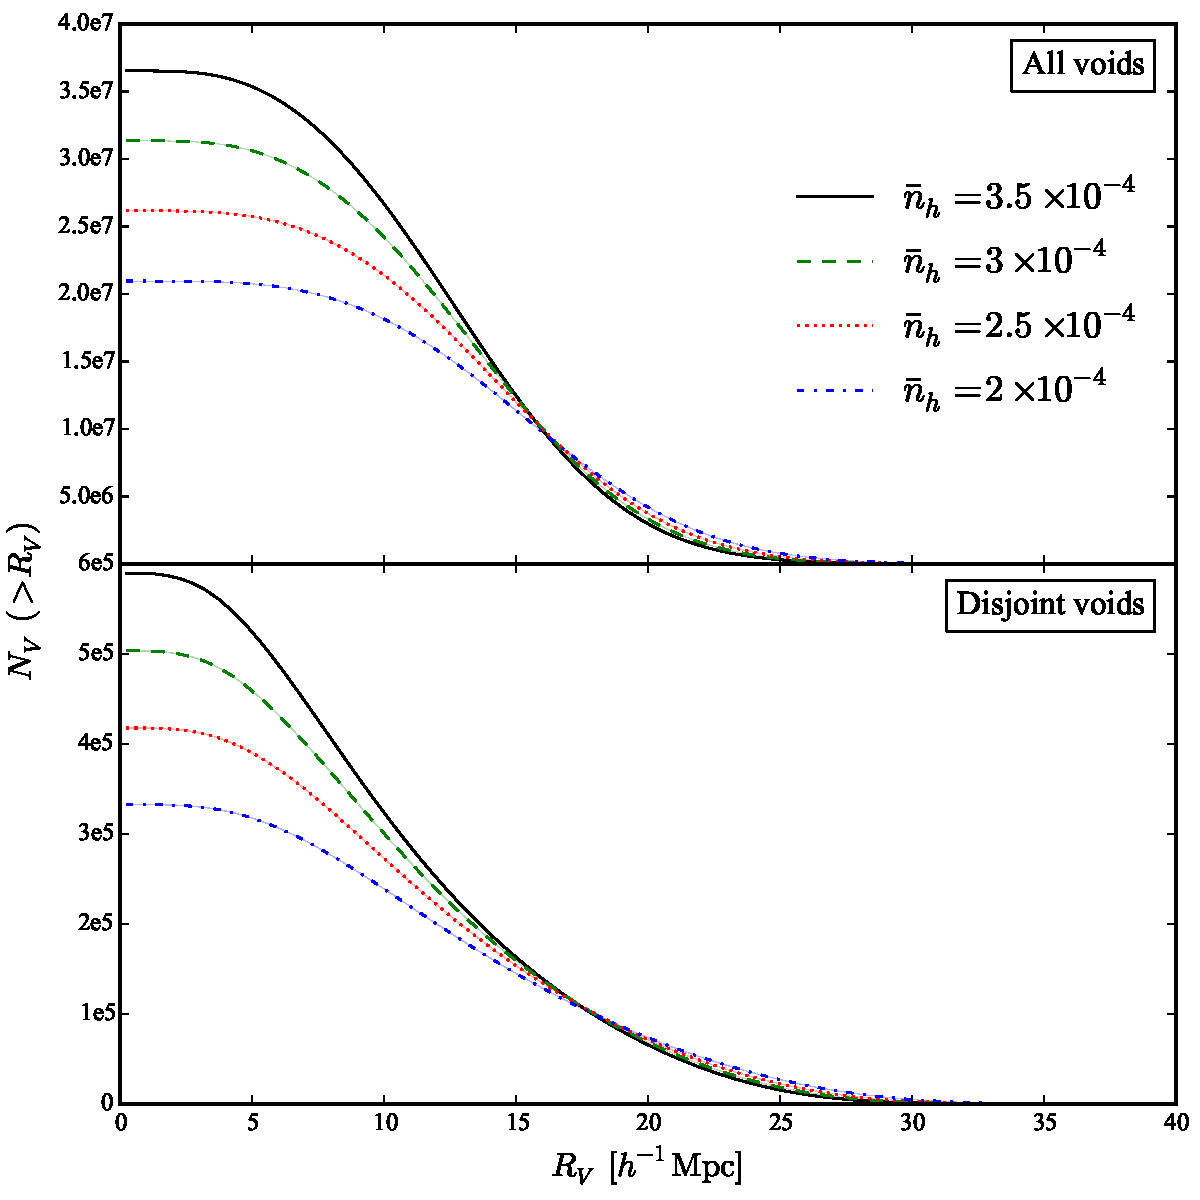
\includegraphics[width=.47\textwidth]{numdens_nmean_cum}
\end{tabular}
\caption{不同颜色的线表示不同数密度的完整模拟暗物质晕表内,巨洞的数量分布(number function,左图)和累积数数量分布(cumulative number function,右图)。阴影区域为1-$\sigma$误差范围,误差非常小所以看上去像实线。(文献 ~\inlinecite{Zhao2016DIVE}中的Figure 4)}
\label{fig:ndens_nmean}
\end{figure}

\begin{figure}
\centering
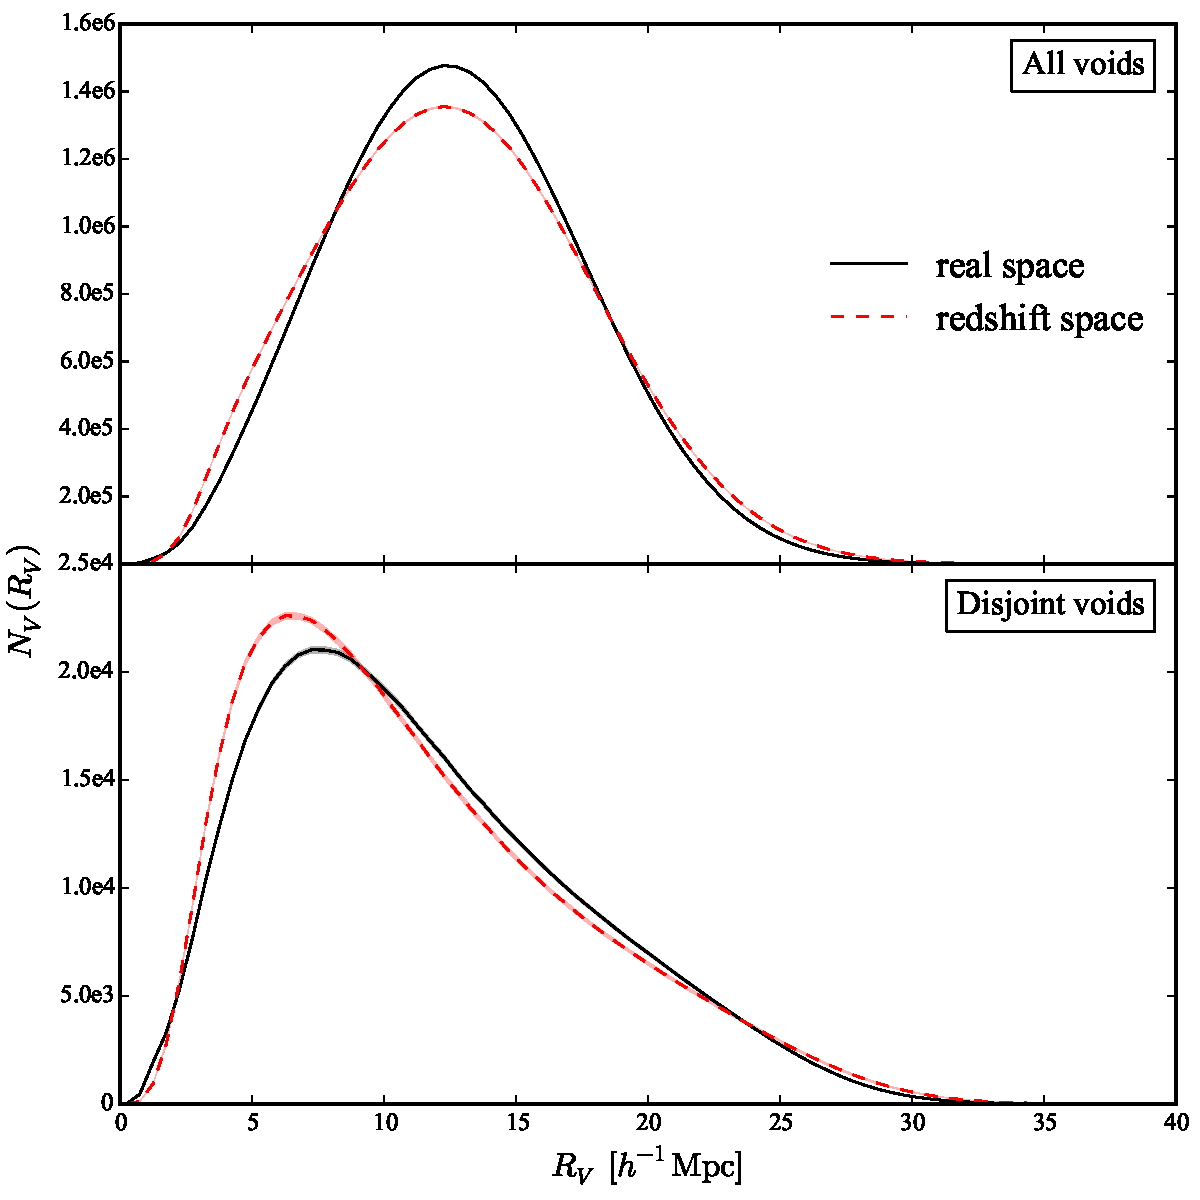
\includegraphics[width=.9\textwidth]{numdens_z}
\caption{实空间与红移空间中DT巨洞和disjoint巨洞的数量分布。1-$\sigma$误差范围非常小,肉眼不可分辨。(文献 ~\inlinecite{Zhao2016DIVE}中的Figure 6)}
\label{fig:ndens_z}
\end{figure}

红移空间的DT巨洞与红移空间的暗物质晕或星系存在一些本质上的区别。对于暗物质晕或星系来说,实空间的位置与红移空间的区别是由于本动速度的存在而使得观测的红移与真实的红移不一致造成的。两者的区别只是视线方向上的位置发生了改变。但是通过DIVE获得的DT巨洞只有球心的位置和半径,没有适当的方式可以被用来定义DT巨洞的速度,因而不能通过DT巨洞在视线方向上的本动速度来将其从实空间转换到红移空间。因为暗物质晕或星系的位置发生了改变,即便可以通过一定的方式将DT巨洞从实空间转换到红移空间,其内部也可能会存在暗物质晕或星系,这与我们对巨洞的定义相矛盾。我们的最终目标是将DIVE用于红移空间中因观测效应而存在各种系统偏差的真实观测数据,不可能直接获得宇宙中星系在实空间中的真实位置。为了保持对巨洞的定义不变,只能将DIVE用于红移空间的完整模拟暗物质晕表来获得红移空间的巨洞数据。而巨洞性质在实空间与红移空间的区别是由暗物质晕或星系的RSD效应间接造成的。

从图~\ref{fig:ndens_z} 的结果可以合理推测,半径较大的DT巨洞或disjoint巨洞,其内部和周围的物质都在朝远离巨洞中心的方向运动,所以在红移空间半径较大的巨洞所在的没有暗物质晕或星系的空旷区域会沿视线方向被拉长,从而使得其中巨洞的半径略微变大。所以红移空间中有更多半径较大的巨洞。非线性RSD效应(Fingers-Of-God,FOG)使得中等半径的巨洞数量减少。因为\textsc{PATCHY}的分辨率为$2.6\,h^{-1}$Mpc,所以结果中更小尺度的RSD效应相比真实情况可能存在一些偏差。

\section{巨洞中心在空间中的分布}

在最早的星系巡天中,发现一些较大的区域内星系的数密度远小于理论预期~\cite{KOS81},或者连续的很大空间内没有观测到任何星系~\cite{LGH86,VGP94},从而发现了巨洞的存在。一般认为在宇宙的高密度区域物质塌缩形成暗物质晕和星系,所以没有暗物质晕或星系的地方可以被认为是宇宙中的低密度区域,也就是巨洞所在的地方。本章我们研究了巨洞中心在空间中相对暗物质晕的分布。

图~\ref{fig:densfield} 展示了实空间完整模拟暗物质晕表的同一区域内,物质密度场、暗物质晕和DT巨洞归一化后的数密度在($x$,$y$)方向上的投影。暗物质晕分布在物质密度场中的高密度区域。所有DT巨洞归一化后的数密度分布与物质密度场也符合的较好,这是因为DT巨洞中半径较小的巨洞占大多数(图~\ref{fig:visual_all})。半径$R \geq 16\,h^{-1}$Mpc的巨洞中心分布在物质密度场中的低密度区域,同时从图~\ref{fig:densfield} 中最下面的图中可以看到,这些巨洞的中心分布在没有暗物质晕的空旷区域,两者共同占据了整个空间。这个结果又一次证明半径$R \geq 16\,h^{-1}$Mpc的DT巨洞中心分布在宇宙低密度区域。

\begin{figure}
\centering
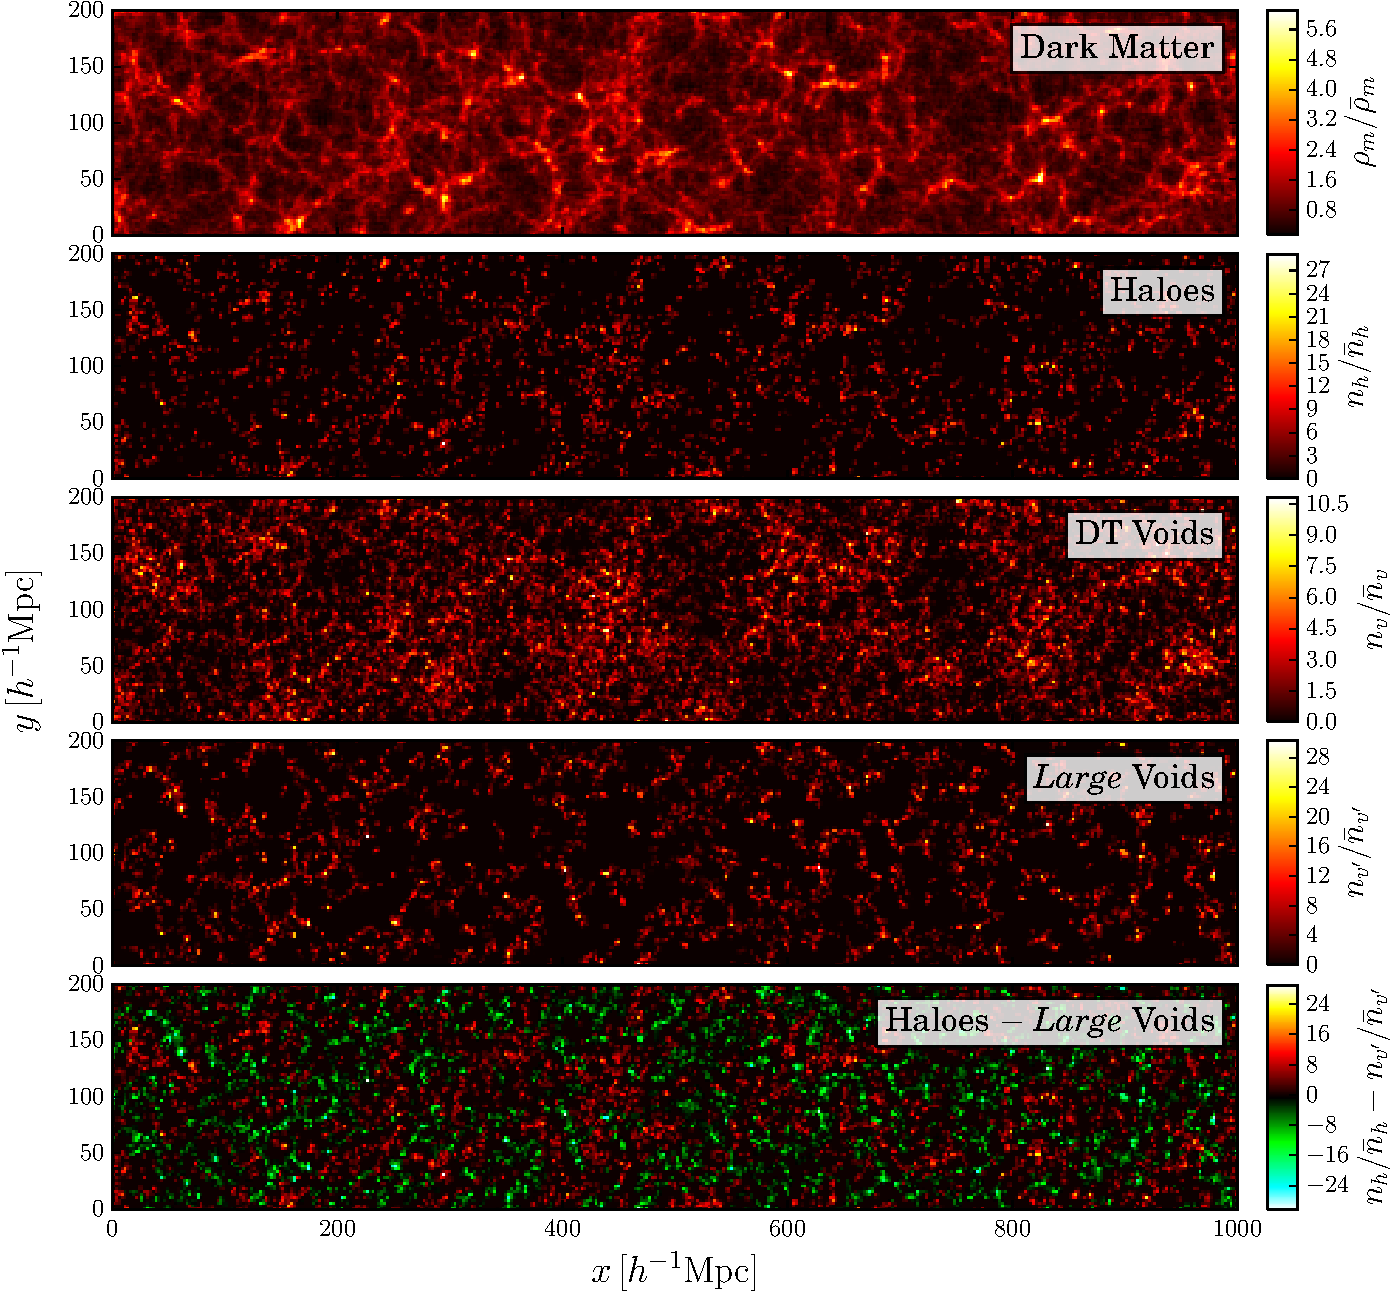
\includegraphics[width=.9\textwidth]{densfield}
\caption{一个完整模拟暗物质晕表的$1000\times500\times50\,h^{-3}\mathrm{Mpc}^3$体积内,物质密度场、暗物质晕(halos)、所有DT巨洞(DT Voids)和半径$R \geq 16\,h^{-1}$Mpc的巨洞(\textit{Large} Voids)相对平均数密度归一化后的数密度分布,最下面的图中为了区别于暗物质晕,\textit{Large} Voids的数密度用负数表示。(文献 ~\inlinecite{Zhao2016DIVE}中的Figure 8)}
\label{fig:densfield}
\end{figure}

\section{巨洞附近的物质密度分布}

上一节我们定性的分析了DT巨洞在物质密度场中的分布,这一节我们定量的分析巨洞中心区域的物质密度及巨洞内部和周围的物质密度轮廓(Density profiles)。

\subsection{巨洞中心的物质密度}

通过\textsc{PATCHY}计算物质密度场时将空间分为$960^3$个网格,分辨率为$2.6\,h^{-1}$Mpc。DT巨洞中心处的物质密度反差$\delta_m$(density contrast,$\delta_m \equiv \rho_m / \bar{\rho}_m - 1$)为离中心最近的一个网格的$\delta_m$。图~\ref{fig:radens} 展示了不同半径DT巨洞在不同$\delta_m$处的数量。大半径的DT巨洞中心的$\delta_m$几乎都很小且平均值小于0,而小半径的DT巨洞中心$\delta_m$普遍很大与暗物质晕的$\delta_m$相当。DT巨洞中心的平均$\delta_m$随着半径的增加而减小。

\begin{figure}
\centering
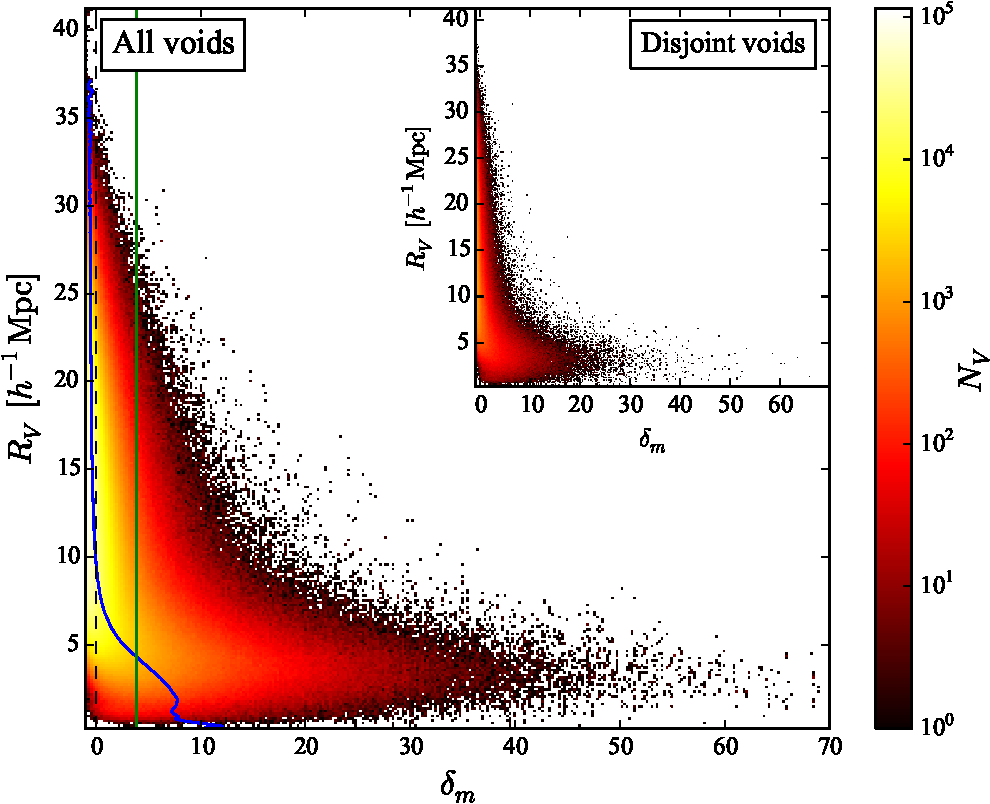
\includegraphics[width=.9\textwidth]{radens}
\caption{不同半径的DT巨洞中心在不同物质密度反差$\delta_m$的数量。蓝色实线表示不同半径DT巨洞中心的平均$\delta_m$,绿色实线是暗物质晕的平均$\delta_m$。(文献 ~\inlinecite{Zhao2016DIVE}中的Figure 9)}
\label{fig:radens}
\end{figure}

\subsection{巨洞的物质密度轮廓}

巨洞的物质密度轮廓可以用于研究不同的引力理论~\cite{Cai2015}。但是很难从观测数据直接获得宇宙的精确物质密度场,巨洞的物质密度轮廓只能通过数值模拟的结果进行研究~\cite{Colberg2005,Ricciardelli2013,Hamaus2014,Nadathur2015}。
%通过重构密度场来定义巨洞的方式(ZOBOV或WVF))可以获得较为准确的物质密度轮廓,但是用其他方法寻找的巨洞的物质密度轮廓可能存在一定的弥散~\cite{Ricciardelli2013}。

DT巨洞具有很高的数密度,因此可以得到比较可靠的物质密度轮廓
%及其弥散
。
因为\textsc{PATCHY}的分辨率为$2.6\,h^{-1}$Mpc,而且本工作最感兴趣的是\textit{voids-in-voids}~\cite{SW04}类巨洞,所以这里只将半径较大的DT巨洞根据半径大小分为5个区间,每个半径区间内每2000个巨洞为一个子样本。在一个完整模拟暗物质晕表中,半径$R \geq 25\,h^{-1}$Mpc的DT巨洞有$\sim$140个子样本,其他较小的半径区间有上千组子样本。将每个子样本的巨洞重叠起来计算其中心到两倍半径处的物质密度轮廓,结果如图~\ref{fig:dens_pro}。DT巨洞的物质密度轮廓的形状与其他工作的结果大体一致,但是DT巨洞的物质密度轮廓对半径更敏感。半径较小的DT巨洞即便中心的$\delta_m$都为正。而且小半径的DT巨洞周围被高密度的“墙”所包围,与其他工作的结果一致~\cite{Paz2013,Hamaus2014}。其他半径区间巨洞的物质密度轮廓都在中心附近为负,在一倍半径处$\delta_m$迅速变大,从负值穿过0变正,更远距离处的$\delta_m$慢慢接近0,也就是平均密度。最大的半径区间内巨洞的$\delta_m$从中心往外一直变大但是始终为负。这一结果也说明半径$R \geq 16\,h^{-1}$Mpc的DT巨洞中绝大部分区域分布在宇宙低密度区域。

\begin{figure}
\begin{tabular}{cc}
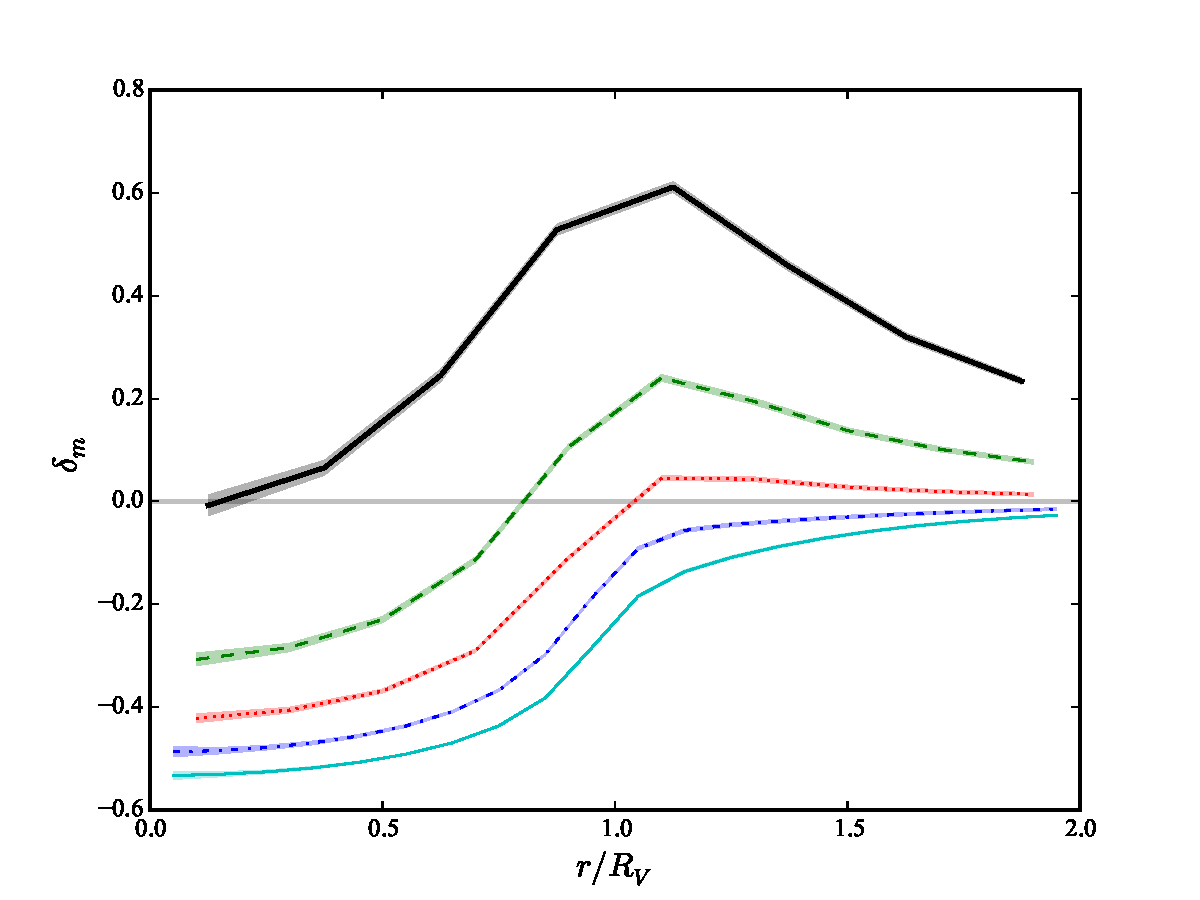
\includegraphics[width=1.\textwidth]{dp_mean}
\end{tabular}
\caption{不同半径区间内所有DT巨洞子样本的平均物质密度轮廓和1-$\sigma$误差范围。$r$是到DT巨洞中心的距离。黑色对应半径范围[8, 12)、绿色对应半径范围[12, 16)、红色对应半径范围[16, 20)、蓝色对应半径范围[20, 25),青色对应半径范围$R \geq 25$,单位为$h^{-1}$Mpc。(文献 ~\inlinecite{Zhao2016DIVE}中的Figure 10)}
\label{fig:dens_pro}
\end{figure}

\section{DT巨洞的动力学特征}

前面研究了静态情况下,DT巨洞所处的物质密度场环境。从整个物质密度场演化的角度来看,初始密度场是比较均匀的,物质不断从低密度区域朝高密度区域聚集,逐渐形成低红移处的宇宙大尺度结构。因此根据动力学特征也可以将宇宙大尺度结构分为不同的成分~\cite{Hahn2007,Forero-Romero2009}。潮汐张量$T_{i j}$是物质密度场$\delta_m$的函数
\begin{equation}
T_{i j} = \frac{\partial^2 \phi}{\partial x_i \partial x_j} 
\end{equation}
其中$\phi$是引力势
\begin{equation}
\nabla^2 \phi = \delta_m 
\end{equation}
三维空间中,潮汐张量的三个本征值(eigenvalues)表示三个方向上的运动方向:如果三个本征值都大于(小于)给定的阈值($\lambda_{\rm th}$)则三个方向都在向里塌缩(向外膨胀),对应的结构为节点knot(巨洞void);如果只有两个(一个)本征值大于阈值($\lambda_{\rm th}$)则两个(一个)方向向里塌缩一个(两个)方向向外膨胀,对应的结构为纤维状结构filament(墙状结构sheet)。

\begin{figure}
\centering
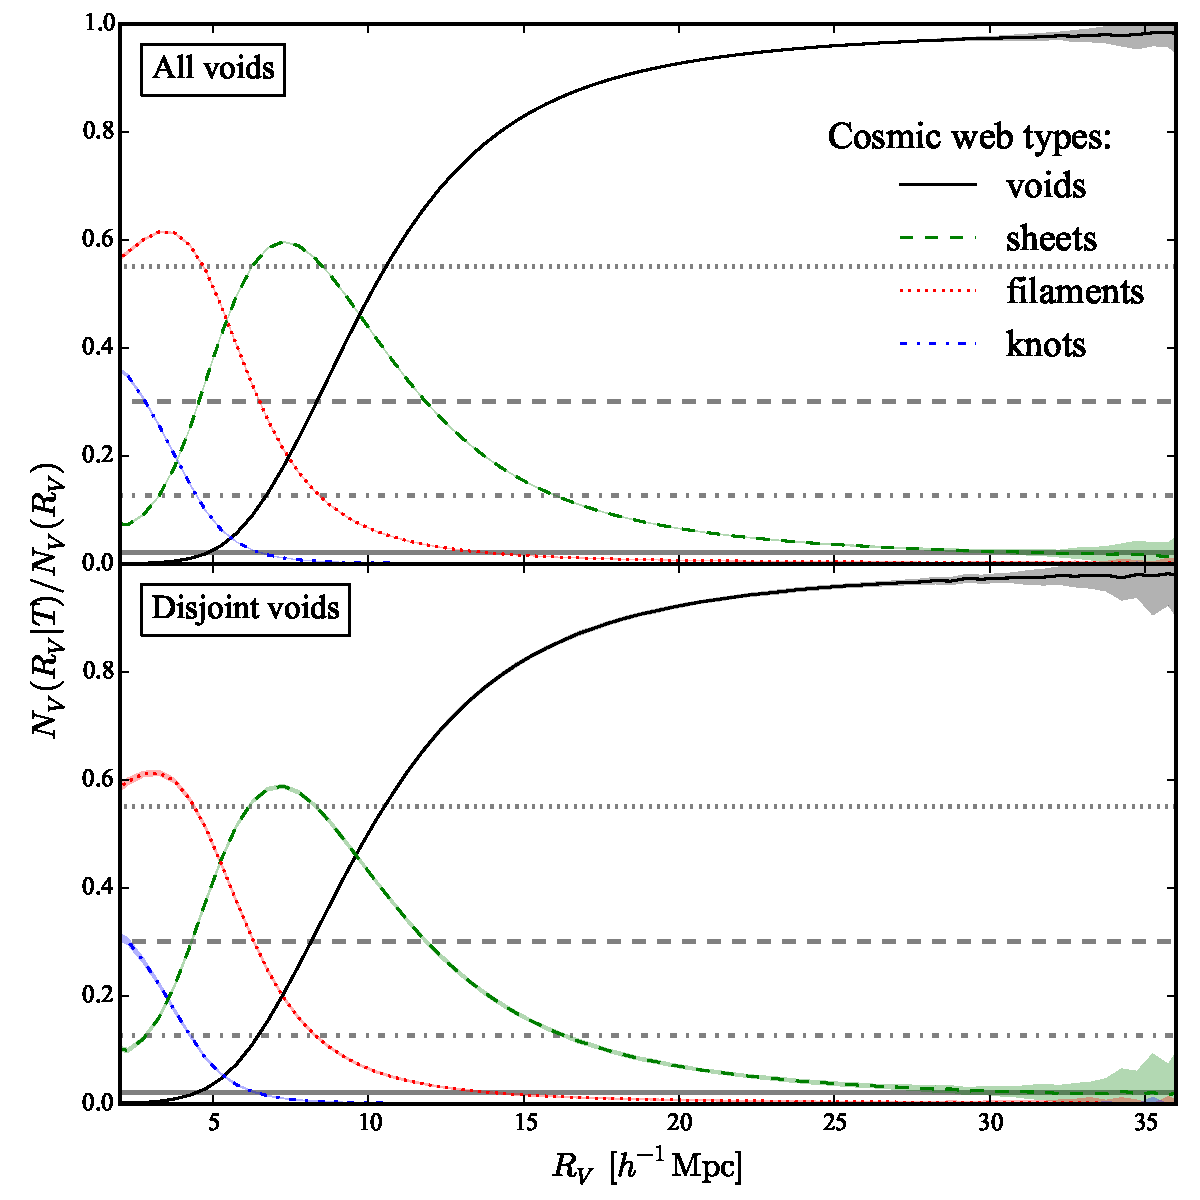
\includegraphics[width=.9\textwidth]{cosmicweb}
\caption{不同半径处DT巨洞按动力学分类后不同成分所占比例。三条水平灰色的线表示将暗物质晕按动力学分类后不同成分所占的比重。阴影区域为100个完整模拟暗物质晕表的1-$\sigma$误差范围。(文献 ~\inlinecite{Zhao2016DIVE}中的Figure 11)}
\label{fig:cosweb}
\end{figure}

通过计算整个物质密度场的潮汐张量$T_{i j}$,并设定阈值$\lambda_{\rm th} = 0.5$,则knot、filament、sheet和void四类结构对应的比重分别为0.6\%、7.6\%、27.8\%和64.0\%。如果将所有DT巨洞根据中心的潮汐张量$T_{i j}$分为不同的结构成分(图~\ref{fig:cosweb}),半径$R \geq 15\,h^{-1}$Mpc的DT巨洞中超过80\%都属于void结构,超过95\%属于void或sheet类结构。这个结果又一次从动力学角度证明了半径$R \geq 16\,h^{-1}$Mpc的DT巨洞分布在宇宙低密度区域。

随着半径减少,DT巨洞属于void结构的越来越少,属于knot结构的越来越多,而其他结构成分所占比例也相应发生变化。半径$R \sim 3.5\,h^{-1}\mathrm{Mpc}$附近的DT巨洞filament结构所占比例最大,与其他工作中filament中星系间典型的距离为$\sim 7\,h^{-1}\mathrm{Mpc}$的结果相一致~\cite{Tempel2014}。

\section{DT巨洞的bias}

\begin{figure}
\centering
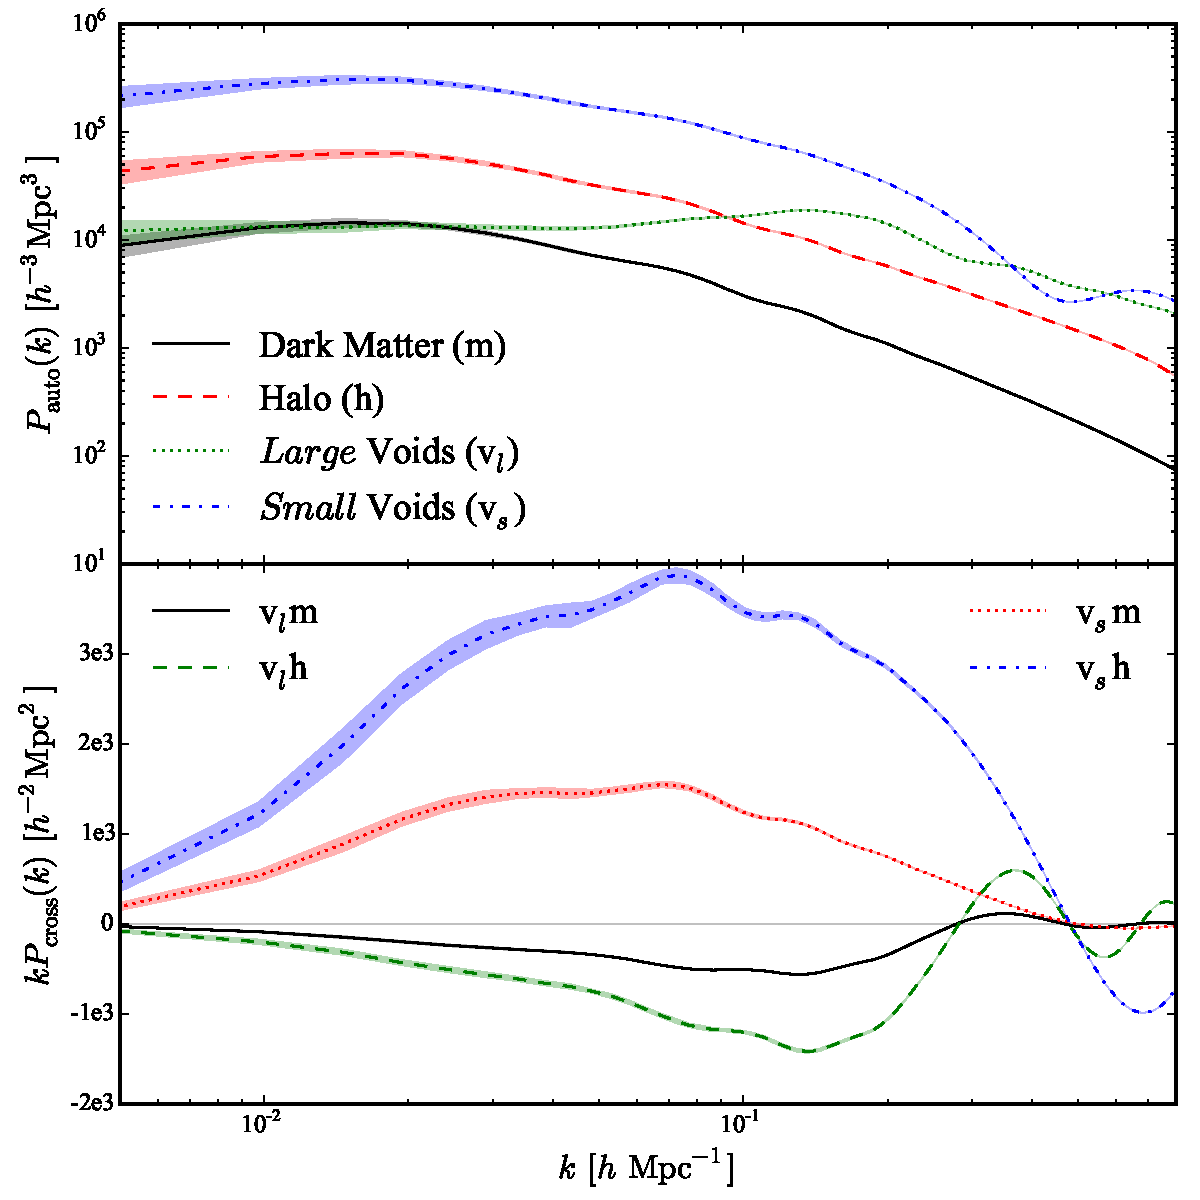
\includegraphics[width=.9\textwidth]{pk}
\caption{上图:Large Voids、Small Voids、暗物质晕(halo)和物质密度场(Dark Matter)的功率谱。下图:Large Voids-暗物质晕、Large Voids-物质密度场、Small Voids-暗物质晕、Small Voids-物质密度场的互功率谱。阴影为100组完整模拟暗物质晕表的1-$\sigma$误差范围。(文献 ~\inlinecite{Zhao2016DIVE}中的Figure 12)}
\label{fig:pk}
\end{figure}

之前的对巨洞的研究中,因为巨洞的数密度很小,很难研究其2PCF或功率谱~\cite{Padilla2005,Patiri2006372,VBT12,CC13,CJS15}。DT巨洞有较大的数密度,可以通过比较DT巨洞的功率谱与物质密度场的功率谱得到DT巨洞的bias。

根据前文的结果,DT巨洞可以分为两类,半径较大的属于\textit{voids-in-voids},半径较小的属于\textit{voids-in-clouds}。根据图~\ref{fig:radens} 和图~\ref{fig:cosweb} 的结果,这一节我们选半径$R \geq 16\,h^{-1}$Mpc的作为较大半径的DT巨洞子样本(Large Voids),半径$R < 8\,h^{-1}$Mpc的作为半径较小的DT巨洞子样本(Small Voids)。

我们分别计算了100组\textsc{PATCHY}完整模拟暗物质晕表的Large Voids、Small Voids、暗物质晕和物质密度场的功率谱(auto-power spectra)和互功率谱(cross-power spectra)。在$k < 0.03\,h\,\mathrm{Mpc}^{-1}$的范围,Large Voids与物质密度场的功率谱幅度几乎相同,Large Voids的bias非常小;而Small Voids的功率谱幅度较大,bias也比较大(如图~\ref{fig:pk} 所示)。因为DIVE找到的Small Voids非常像星系团(cluster)~\cite{Marinoni2002},所以Small Voids与暗物质晕的功率谱在$k < 0.1\,h\,\mathrm{Mpc}^{-1}$范围内整体的形状非常相似,而Small Voids的bias比暗物质晕的更大。

\begin{figure}
\centering
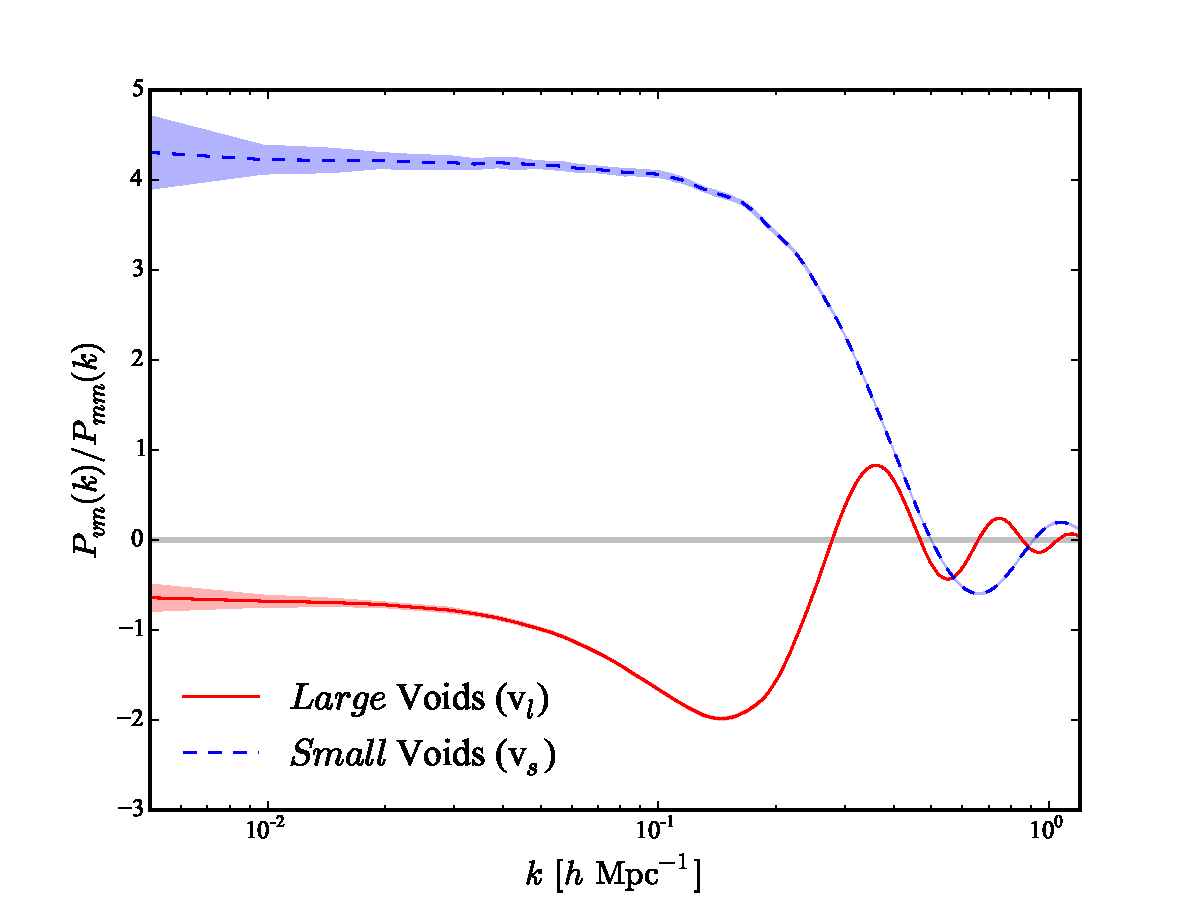
\includegraphics[width=.9\textwidth]{bias_pk}
\caption{Large Voids和Small Voids的bias。阴影区域为100个完整模拟暗物质晕表的1-$\sigma$误差范围。(文献 ~\inlinecite{Zhao2016DIVE}中的Figure 13)}
\label{fig:bias_dp}
\end{figure}

下面我们在线性尺度定量的估算一下Large Voids和Small Voids的bias:
\begin{equation}
b_m (k) = \frac{P_{vm}(k)}{P_{mm}(k)}
\end{equation}
其中$P_{vm}(k)$是DT巨洞和物质密度场的互功率谱,$P_{mm}(k)$物质密度场的功率谱(图~\ref{fig:bias_dp})。在在$k < 0.03\,h\,\mathrm{Mpc}^{-1}$的范围Large Voids和Small Voids的bias几乎不变,Large Voids的bias约等于-0.7,Small Voids的bias约等于4.2(是LRG bias的两倍~\cite{Tegmark2006})。
